\section{Aus dem Leben eines Erstsemesters}

4:30 Uhr: Der ohrenbetäubende Lärm des Weckers reißt mich aus dem Schlaf. Ich werfe die Bücher beiseite und springe vom
Schreibtischstuhl auf. Das war eine erholsame Nacht, ich fühle mich wie neugeboren. Wo ist nur mein Theo-Zettel hin? Ich hab` doch gestern Abend noch bis um 3 dran gearbeitet? Wie jede Nacht. Tag und Nacht!

Im Traum ist mir doch glatt die Lösung der verdammt inhomogenen Differentialgleichung 25.ter Ordnung mit frequenzabhängigen Dispersionsrelationen bei nichttrivialen Randbedingungen eingefallen! Und das im Lagrange-Formalismus! Ach, da ist der Theo-Zettel ja. Auf dem Boden. Ich war nicht kräftig genug, den Batzen Papier auf den Schreibtisch zu heben. Außerdem wäre der Tisch sowieso zusammengebrochen. Da rechne ich doch geschwind mal weiter, ich habe ja noch eine halbe Stunde Zeit.

5:00 Uhr: Ich treffe mich mit drei Kommilitonen, um die
Mathe-Vorlesung vorzubereiten. Heute geht es um die Approximation differenzierbarer Funktionen durch Anwendung des Virialsatzes auf die Säkulardeterminante. Ein spannendes Thema, das man gleich benutzen kann, den Lemaître-Eddington-Kosmos des Reflexklystrons im Lobatschewsky-Bolyai-Raum zu veranschaulichen. Heute wird ein schöner Tag.

6:00 Uhr: Zeit für die fünf Protokolle, die ich heute abgeben muss. Eigentlich ist das gemein - fünf Protokolle. Von gestern auf heute. Aber wer damit nicht klar kommt, der gehört hier halt nicht hin. Die Leute findet man dosenstapelnderweise beim Aldi. Oder bei den BWL--ern.

7:00 Uhr: Zeit für Frühstück.

7:01 Uhr: Ah, jetzt geht`s mir gut. Ab zu den Informatikern, ein Nebenfach will schließlich auch gepflegt werden. Ich wundere mich ja heute noch wie man vier Programmiersprachen in drei Tagen lernen kann, aber irgendwie ging`s!

7:30 Uhr: Ich muss noch die drei Kilo Papier besorgen, die ich für die Vorlesung brauche. Der fleißige Physikstudent schreibt
schließlich mit. Außerdem, ist es Zeit für die tägliche
Koffeinspritze.

7:45 Uhr: Ab in den Hörsaal, sonst sitz` ich schon wieder nur in der zweiten Reihe. Juhu, diesmal hab ich noch einen Platz in der ersten Reihe ergattern können, ein bisschen am Rand, aber die anderen waren einfach schon `ne Stunde früher als ich.

8:15 Uhr: Der Messias betritt den Saal. Er erleuchtet uns die
folgenden zwei Stunden mit reinstem, gesegnetem Wissen\ldots

10:15 Uhr: Experimentalphysik. Das finde ich langweilig, weil
trivial.

11:15 Uhr: Eine Freistunde! Heissa! Endlich kann ich in Ruhe ganz alleine rechnen. Ich hab doch gesagt, dass ein schöner Tag wird! Ich versteh nicht, wie andere essen gehen können. Was soll das? Stümper\ldots

12:15 Uhr: Theoretische Physik, die Königin der Wissenschaften. Hier ist man Gott am nächsten! Alle gucken so verwirrt, als ob sie es nicht verstanden hätten. Dabei sind wir doch erst bei Seite 798 des Buches, und es sind erst zwei Wochen rum. Wie können die eigentlich die täglichen fünfzehn Aufgaben schaffen, wenn sie nicht mal die Vorlesung verstehen? Oder vielleicht schauen sie auch nur gelangweilt. Ich muss auch zugeben, eine Geschwindigkeit von einer Tafel in zwei Minuten ist schon etwas lahm. Der war auch mal schneller.

13:00 Uhr: Fachbereichsratssitzung. Etwas politisches Engagement wird von einem Erstsemester schließlich auch erwartet.

22:30 Uhr: Nach einem Diskussionsmarathon darüber, ob Professor Greiner wegen seines neuen Ehrendoktors heute den Platz am Kopfende des Tisches bekommt oder doch neben dem Aquarium sitzen muss, mussten wir mangels einer alle zufrieden stellenden Lösung die Sitzung vorzeitig beenden. Glücklicherweise, denn sonst hätte ich nicht die Zeit gefunden, das Buch \glqq Corund methods for the solution
of the cyropolus-problem with the leptonic Purcell-Planck-equation\grqq  durchzulesen, das ich doch für die Aufgaben brauche.

23:30 Uhr: Puh, geschafft. Wenn man wöchentlich ein Bibliotheksregal durcharbeiten muss, lernt man das schnelle Lesen ganz gut. Jetzt muss ich aber wirklich meine Theo-Aufgaben weiter rechnen! 

4:30 Uhr: Zeit zu schlafen, leider, aber was sein muss, muss sein.

4:45 Uhr: Endlich, ein neuer interessanter, spannender, aufregender Physiker-Tag beginnt\ldots
\begin{figure}[!b]
 \begin{center}
  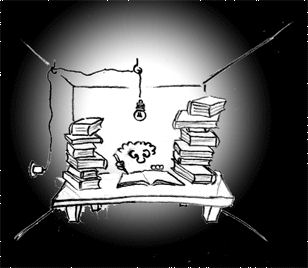
\includegraphics[width=.8\textwidth]{bilder/ersti.jpg}
 \end{center}
\end{figure}

\von{Sascha (der hat jetzt seinen 20. Herzinfarkt hinter sich\ldots) und Julia}
